
\documentclass[12pt]{amsart}   % LaTeX with AMS style; 12 point for old eyes

\usepackage{amssymb,amsfonts}   % For better support of math
\usepackage{graphicx}	        % Enable for eps and pdf figures, if they occur
\usepackage{hyperref}           % Enable embedded hyperlinks.
\usepackage[bottom]{footmisc}
\usepackage{listings}
\usepackage[most]{tcolorbox}
\usepackage{inconsolata}

% Commands to force sequential numbering:

\newtheorem{theorem}{Theorem}[section]
\newtheorem{proposition}[theorem]{Proposition}
\newtheorem{lemma}[theorem]{Lemma}
\newtheorem{definition}[theorem]{Definition}
\newtheorem{examples}[theorem]{Examples}
\newtheorem{remarks}[theorem]{Remarks}
\newtheorem{corollary}[theorem]{Corollary}
\newtheorem{remark}[theorem]{Remark}
\newtheorem{example}[theorem]{Example}
\newtheorem{conjecture}[theorem]{Conjecture}

\begin{document}

\title[CSE380 Assignment 4]{CSE380 Tools and Techniques for Computational Science Assignment 4 
[Modeling document]} 
% the first [...] gives a brief version of the title, which is long!
 
\author{Mohammad Afzal Shadab}\email{mashadab@utexas.edu}
\date{\today}              % or an actual date


\newcommand{\C}{\mathbb C} % blackboard bold , for ``complex,'' etc
\newcommand{\R}{\mathbb R} 
\newcommand{\Z}{\mathbb Z}
\newcommand{\Q}{\mathbb Q}
\newcommand{\N}{\mathbb N}

\begin{abstract}
This is a \textit{modeling document} for the application to solve the steady-state heat equation in one- and two-dimensions. The document highlights the governing equations, boundary conditions, numerical approximations, and high-level pseudocode implemented in the solver.  
\end{abstract}

\maketitle

\section{Governing equations and boundary conditions\label{sec:goveqn}}
The steady-state heat equation with a constant coefficient in two dimensions is given by:
\begin{equation} \label{eq:1}
    \boxed{-k \nabla^2T(x,y) = q(x,y) \quad \forall \Omega\in[0,L]\times[0,H]}
\end{equation}
where $k$ is the thermal conductivity (W/K), $T(x,y)$ is the material temperature (K), $q(x,y)$ is a heat source term (W/m$^2$) and $\Omega \subset \mathbb{R}^2$ is the domain. This is Poisson equation which is a type of elliptic partial differential equations. This linear boundary value problem is subjected to either \textit{Dirichlet boundary conditions} ($T$ specified) following \textit{maximum principle} or combinations of \textit{Neumann} ($\nabla T$ specified), \textit{Dirichlet} and \textit{Robin boundary conditions}. To begin with, let's specify Dirichlet boundary conditions:
\begin{eqnarray}
T(0,y) &=& T_{analytical}(0,y) \nonumber\\
T(L,y) &=& T_{analytical}(L,y)\\
T(x,0) &=& T_{analytical}(x,0)\nonumber\\
T(x,H) &=& T_{analytical}(x,H)\nonumber
\end{eqnarray}
where $T_{analytical}$ is evaluated using MASA.
\section{Assumptions \label{sec:assumptions}}
We'll start with the assumptions for the derivation of equation \ref{eq:1} from the law of conservation of energy in Eulerian framework \ref{eq:3} \cite{oden2011introduction}:
    \begin{equation} \label{eq:3}
        \frac{ \partial }{ \partial t }{(\rho e) + \nabla \cdot(\rho e \textbf{u}) = \textbf{T}:\textbf{D} -\nabla \cdot \textbf{q} + r}
    \end{equation}
where $e$ is internal energy per unit mass, $\textbf{T}:\textbf{D}$ is the strain heating, $\textbf{q}$ is the heat flux and $r$ is the volumetric source / sink. 
\begin{itemize}
\item Continuum assumption
    \item Steady-state ($\partial(.) / \partial t = 0$)
    \item No advection $\textbf{u}=\textbf{0}$
    \item No source/sink term $r=0$
    \item Validity of \textit{Fourier's law of heat conduction}, i.e., $\textbf{q} =-k \nabla T$
    \item No strain heating, i.e., $\textbf{T : D}=0$, where $\textbf{T}$ is the stress tensor and $\textbf{D}$ is the deformation tensor
    \item Constant coefficient of thermal conductivity $k$
\end{itemize}

Moving towards the assumptions to make the numerical implementation easier:
\begin{itemize}
    \item Square domain $L\equiv H$
    \item Uniform grid, i.e. $N_x=N_y=N$, where $N_x$ and $N_y$ are the cells in x and y directions respectively. So, $\Delta x = \Delta y = h$
    \item The Dirichlet boundary conditions are implemented in form of constant temperatures in the ghost cells adjacent to a corresponding boundary, i.e., $T_{0,1}=T_{analytical}(x_0,y_1)$
\end{itemize}

\section{Nomenclature}
For 1D, the mesh numbering is simple and straight forward, as shown in figure \ref{fig:1}. The scheme is cell based, where cell centers $(x_c,y_c)$ are referred to most of the times.
\begin{figure}[b!]
    \centering
    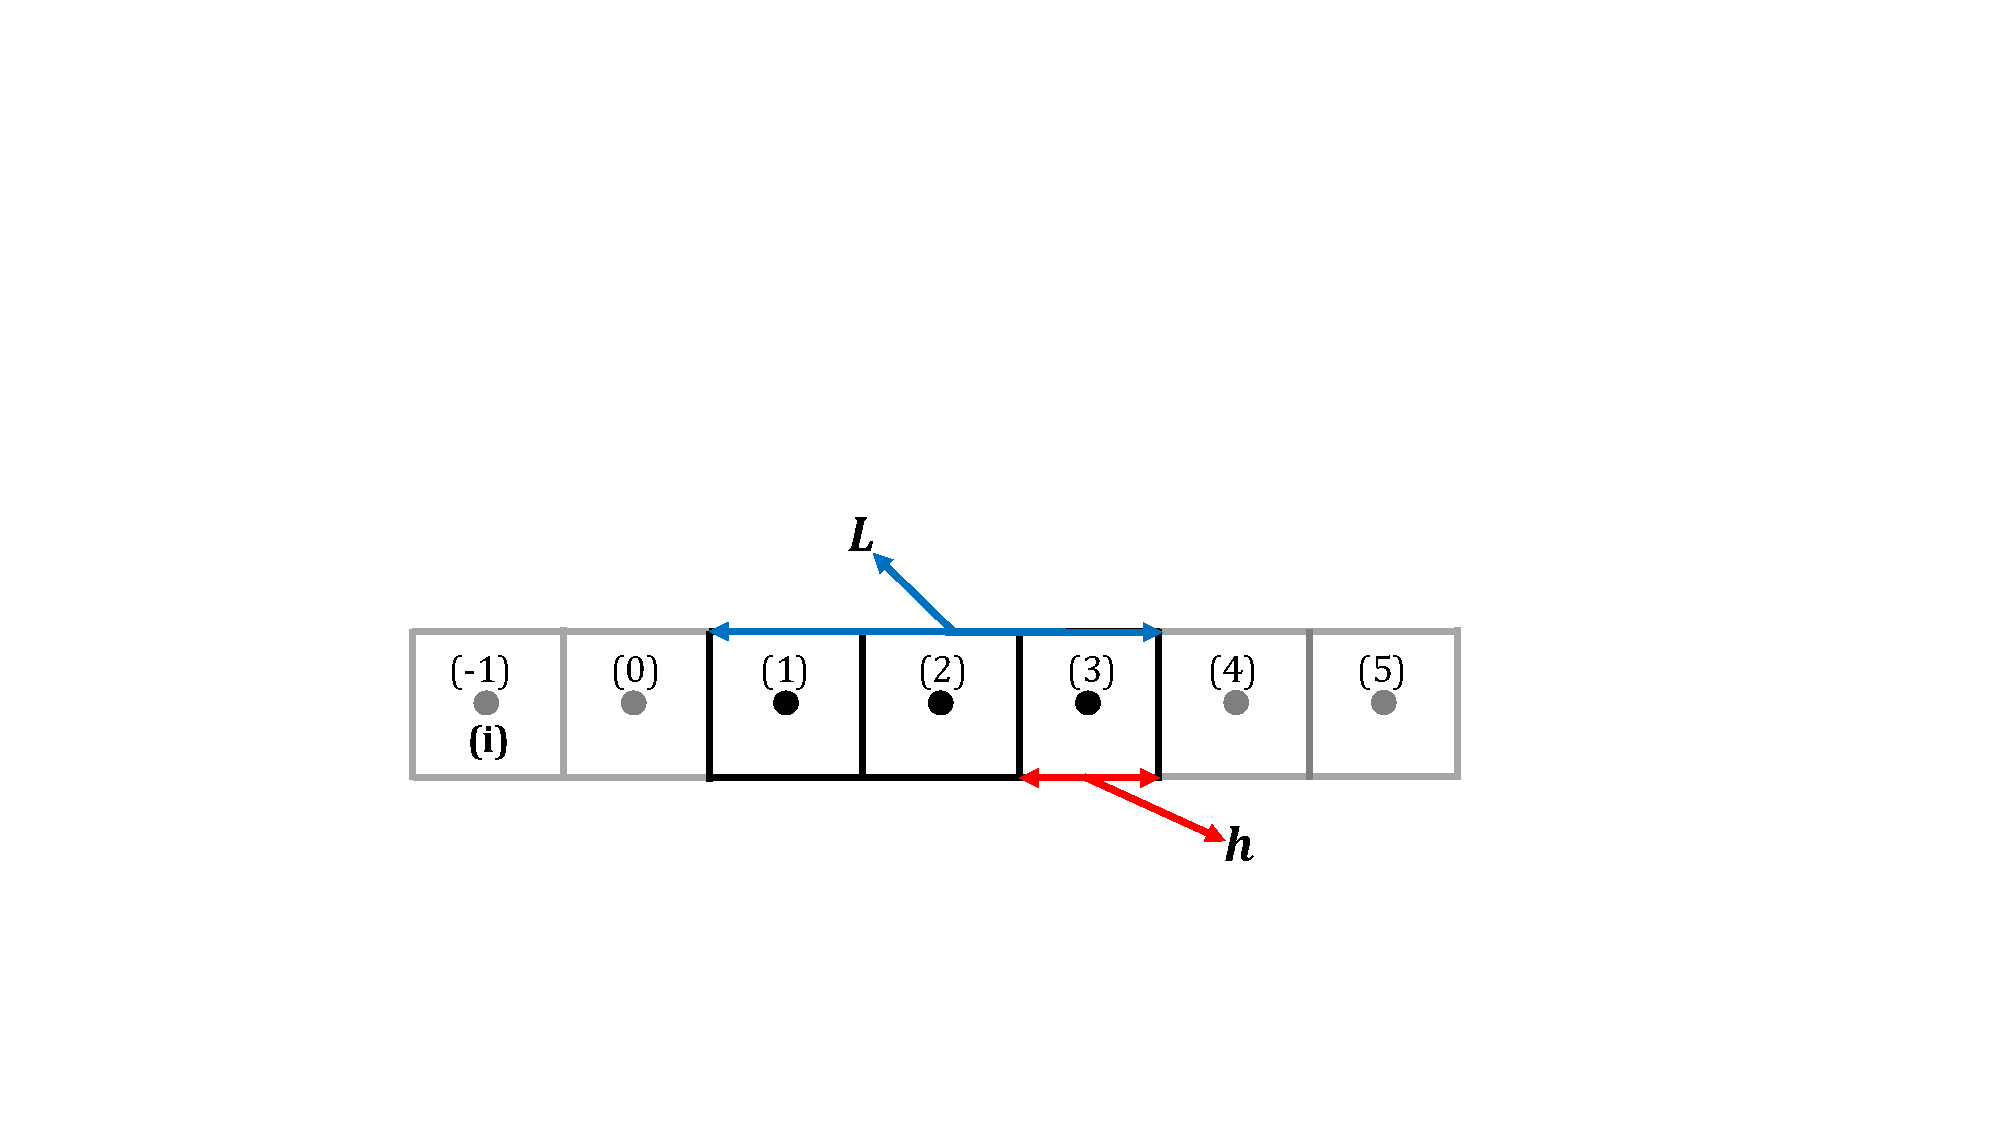
\includegraphics[width=\linewidth]{fig1_1D.pdf}
    \caption{1D mesh with 3 cells, grey ghost cells, and $i$ indexing}
    \label{fig:1}
\end{figure}

For 2D mesh, the situation is slightly sophisticated as two indices $(i,j)$ come to picture correspondingly in x and y directions illustrated in figure \ref{fig:2}. So, using a new numbering system for converting $(i,j)$ into one index $k$ which spans x direction cells first then marches in y direction, 
\begin{eqnarray}
k &=& i+(j-1)N_x, & k \in\{1,2,...,N_x*N_y\} \nonumber\\
k\%N_x &=& i & \text{(Remainder)}  \\
k/N_x &=& j-1 &\text{(Integer division)}  \nonumber 
\end{eqnarray}

\begin{figure}
    \centering
    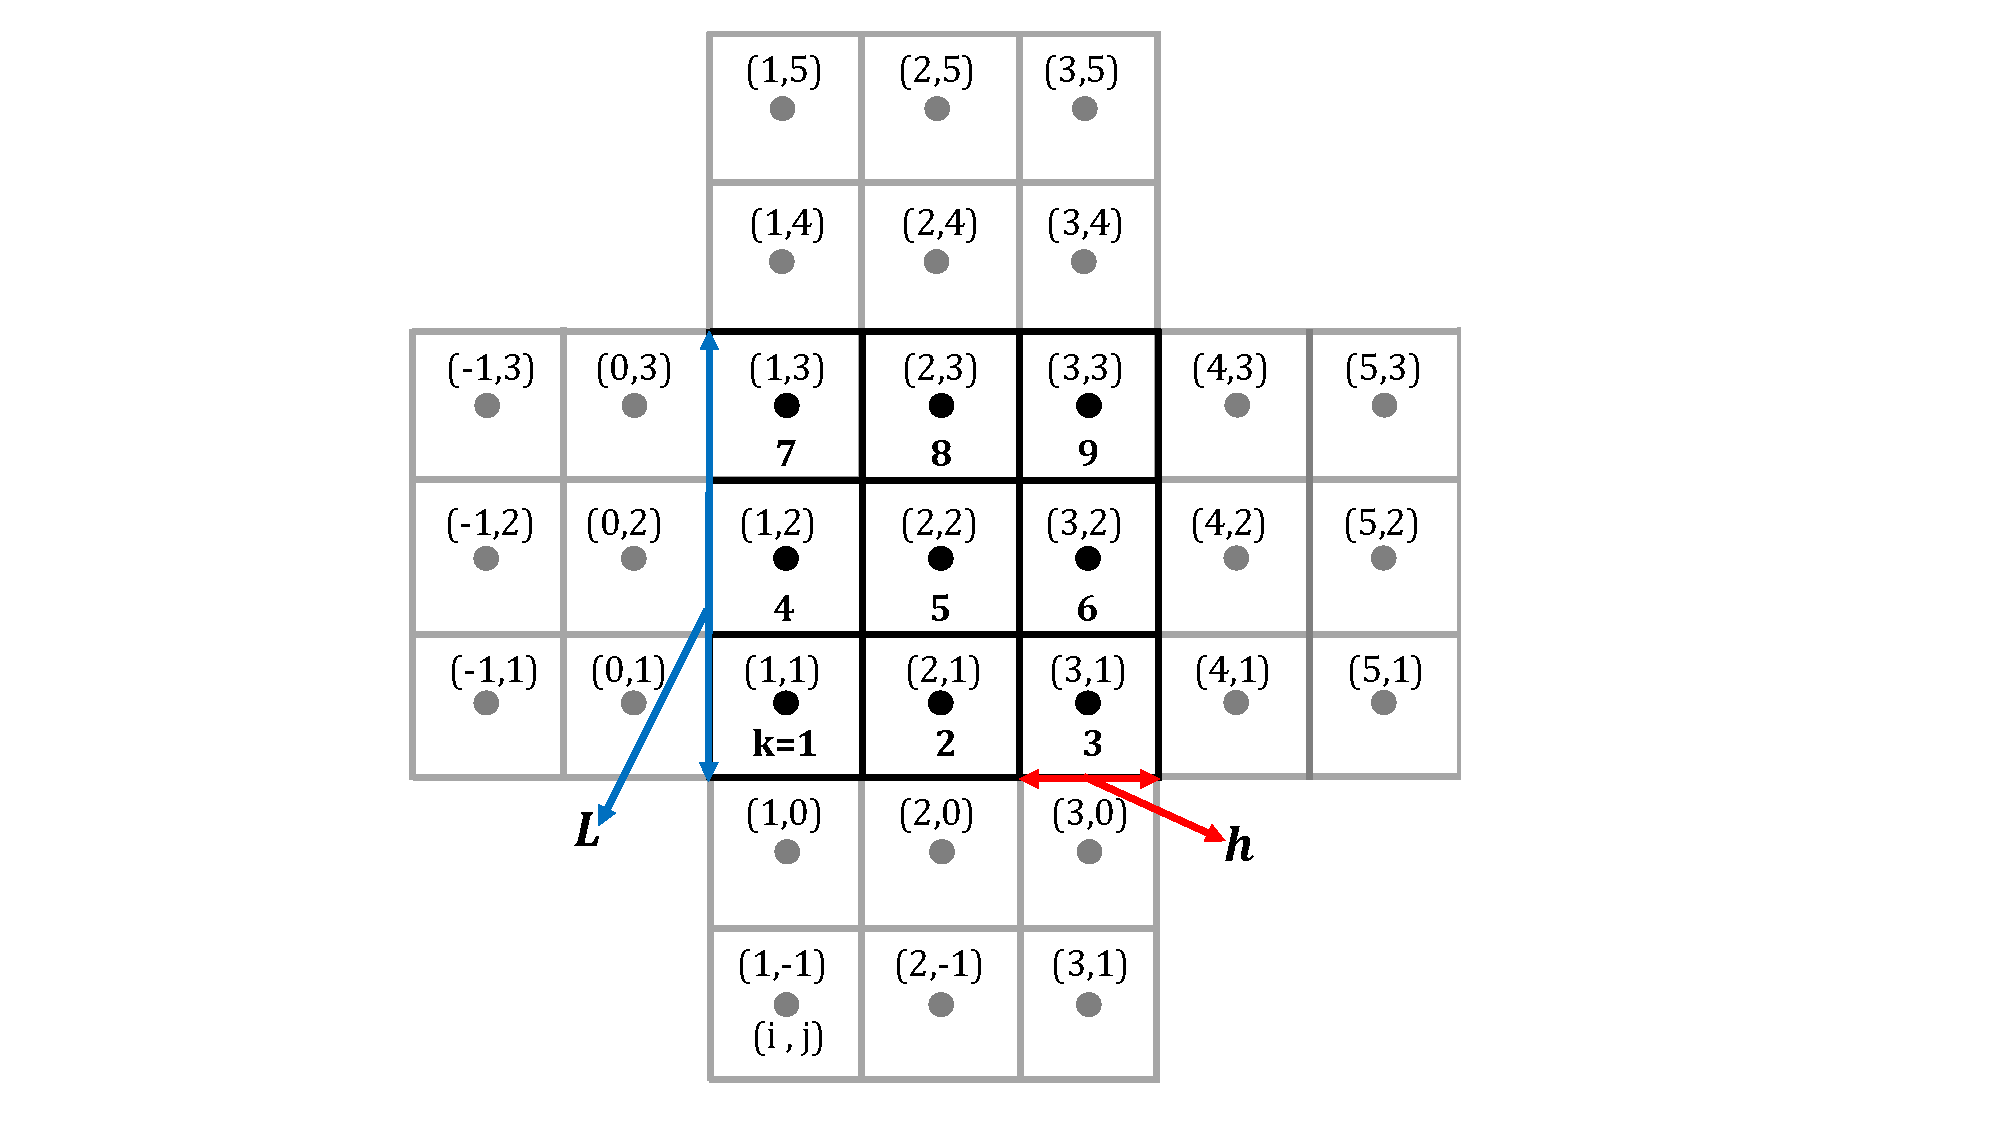
\includegraphics[width=\linewidth]{fig2_2D.pdf}
    \caption{2D $3\times3$ uniform mesh with grey ghost cells, $(i,j)$ indexing, and universal $k$ indexing}
    \label{fig:2}
\end{figure}
Be careful as the ghost cells are not considered in the $k$ numbering and $(i,j)$ points referring to ghost cell centers indices.

\section{Numerical Methods}
Finite difference approximation has been implemented considering the ease in implementation when compared with other discretization methods such as finite volumes, finite element, etc \cite{quarteroni2010numerical}. Rewriting equation \ref{eq:1} in expanded form for 1D
\begin{equation} \label{eq:5}
    -k \frac{\partial^2 T(x) }{\partial x^2} = q(x)
\end{equation}
and for 2D
\begin{equation}\label{eq:6new}
    -k \bigg(\frac{\partial^2 T(x,y) }{\partial x^2}+\frac{\partial^2 T(x,y) }{\partial y^2} \bigg) = q(x,y)
\end{equation}

\subsection{Second order finite difference approximation}
Using the Taylor's expansion, the second order central difference approximation for second order derivative in x direction can be written
\begin{equation}\label{eq:6}
 \frac{ \partial^2 T}{\partial x^2}=\frac{T_{i+1} -2T_{i} + T_{i-1}}{\Delta x^2}+\mathcal{O}(h^2)  
\end{equation}
where subscript $i$ is the cell centered value of cell $i$.
\subsubsection{1D} Equation \ref{eq:6} can be substituted into equation \ref{eq:5}, to give
\begin{equation}
-k \Bigg(\frac{T_{i+1} -2T_{i,j} + T_{i-1}}{\Delta x^2} \Bigg)+\mathcal{O}(h^2) = q_i
\end{equation}
Inserting $\lambda = -k/\Delta x^2$ and dividing by $\lambda$, we get
\begin{equation}
{T_{i+1} -2T_{i} + T_{i-1}} +\mathcal{O}(h^4) = q_i/\lambda
\end{equation}
Neglecting the truncation error $\mathcal{O}(h^4)$ and writing in matrix form for a 3 cell grid shown in figure \ref{fig:1} after implementing the penalty approach for the boundary terms, we get
\begin{equation}
 \begin{pmatrix}
-2 & 1 &  \\
1 & -2 & 1 \\
 & 1 & -2 \\
\end{pmatrix} \begin{bmatrix}
T_{1}\\
T_{2}\\
T_{3}\\
\end{bmatrix} =
\begin{bmatrix}
{q_{1}}/{\lambda}-T_{0}\\
{q_{2}}/{\lambda}\\
{q_{3}}/{\lambda}-T_{4}\\
\end{bmatrix} \Rightarrow \textbf{AT=B}
\end{equation}

For a $N$-cell grid, the matrix equation takes the following form, 
\begin{equation}
\textbf{A}=\begin{pmatrix}
-2 & 1 & & &&\\
1 & -2 & 1 && & \\
& 1 & -2 & 1 && \\
&  & \ddots & \ddots & \ddots& \\
&   && 1 &-2 &1\\
&   & & &1 &-2\\
\end{pmatrix}, \textbf{T}=\begin{bmatrix}
{T_{1}}\\
{T_{2}}\\
\vdots\\
{T_{N-1}}\\
{T_{N}}\\
\end{bmatrix}, \textbf{B}=\begin{bmatrix}
{q_{1}}/{\lambda}-T_{0}\\
{q_{2}}/{\lambda}\\
\vdots\\
{q_{N-1}}/{\lambda}\\
{q_{N}}/{\lambda}-T_{N+1}\\
\end{bmatrix}
\end{equation}
So, the resulting matrix \textbf{A} is tridiagonal (\textcolor{red}{3 diagonals}).
\begin{equation}
\textbf{A}=\begin{pmatrix}
\times & \times & & &&\\
\times & \times & \times && & \\
& \times & \times & \times && \\
&  & \ddots & \ddots & \ddots& \\
&   && \times & \times &\times\\
&   & & &\times &\times\\
\end{pmatrix}\end{equation}

\subsubsection{2D}
We can write
\begin{equation}
    -k \Bigg(\frac{T_{i+1,j} -2T_{i,j} + T_{i-1,j}}{\Delta x^2}+\frac{T_{i,j+1} -2T_{i,j} + T_{i,j-1}}{\Delta y^2} \Bigg)+\mathcal{O}(h^2) = q_{i,j}
\end{equation}
where $i$ and $j$ are the positions of cell center in x and y directions. Implementing, $\Delta x = \Delta y = h$ from assumptions and $-k/h^2 = \lambda$
\begin{equation}
     T_{i+1,j} + T_{i-1,j}+T_{i,j+1} + T_{i,j-1} -4T_{i,j} +\mathcal{O}(h^4) = q_{i,j} / \lambda
\end{equation}
Since we have disconnected elements at $i=1,N$, using $k$ notation for same row, i.e, when $(k+1)/N = (k-1)/N = k/N = i$
\begin{equation}
     T_{k,k+1} + T_{k,k-1}+T_{k,k+N_x} + T_{k,k-N_x} -4T_{k,k} +\mathcal{O}(h^4) = q_{k} / \lambda \quad \text{(for same row)}
\end{equation}
Using penalty approach for boundary terms, for a $3\times3$ uniform grid, the resulting matrix equation takes the form\\
\begin{eqnarray}
\begin{pmatrix}
-4 & 1 &  & 1 &&&\\
1 & -4 & 1 &  & 1 &&\\
 & 1 & -4 &  & &1&\\
1 &  &  & -4 & 1&&1\\
 & 1 &  & 1 &-4&1&&1\\
 &  & 1 & &1&-4&&&1\\
 &  &  &1 && &-4&1\\
 &&  &  &1 && 1&-4&1 \\
 &&&  &  &1 && 1&-4
\end{pmatrix} \begin{bmatrix}
T_{1}\\
T_{2}\\
T_{3}\\
T_{4}\\
T_{5}\\
T_{6}\\
T_{7}\\
T_{8}\\
T_{9}\\
\end{bmatrix} &=&
\begin{bmatrix}
{q_{1}}/{\lambda}-T_{1,0}-T_{0,1}\\
{q_{2}}/{\lambda}-T_{2,0}\\
{q_{3}}/{\lambda}-T_{4,1}-T_{3,0}\\
{q_{4}}/{\lambda}-T_{0,2}\\
{q_{5}}/{\lambda}\\
{q_{6}}/{\lambda}-T_{4,2}\\
{q_{7}}/{\lambda}-T_{0,3}-T_{1,4}\\
{q_{8}}/{\lambda}-T_{2,4}\\
{q_{9}}/{\lambda}-T_{4,3}-T_{3,4}\\
\end{bmatrix} \nonumber \\
\Rightarrow \textbf{AT}&=&\textbf{B}
\end{eqnarray}
For a $N\times N$ grid, the matrix equation takes the following form \ref{eq:16},
\begin{eqnarray} \label{eq:16}
\hspace{-3cm}
\begin{pmatrix}
-4 & 1 & \Leftarrow(N-1)\Rightarrow & 1 &&&\\
1 & -4 & 1 & \Leftarrow(N-1)\Rightarrow & 1 &&\\
 & 1 & -4 & 1 & &\ddots&\\
1 & \Leftarrow(N-1)\Rightarrow & 1 & \ddots &\ddots&&1\\
 & 1 &  & \ddots &\ddots&1&\\
 &  & \ddots & &1&-4&1\\
 &  &  &1 &\Leftarrow(N-1)\Rightarrow& 1&-4\\
\end{pmatrix} \begin{bmatrix}
T_{1}\\
T_{2}\\
T_{3}\\
\vdots \\
T_{N}\\
T_{N+1}\\
\vdots\\
T_{N*N-1}\\
T_{N*N}\\
\end{bmatrix}  = \nonumber \\
\begin{bmatrix}
{q_{1}}/{\lambda}-T_{1,0}-T_{0,1}\\
{q_{2}}/{\lambda}-T_{2,0}\\
{q_{3}}/{\lambda}-T_{3,0}\\
\vdots\\
{q_{N}}/{\lambda}-T_{N+1,1}-T_{N-1,0}\\
{q_{N+1}}/{\lambda}-T_{0,2}\\
\vdots\\
{q_{N*N-1}}/{\lambda}-T_{N-1,N+1}\\
{q_{N*N}}/{\lambda}-T_{N,N+1}-T_{N+1,N}\\
\end{bmatrix} \nonumber \\
\hspace{-2cm} \Rightarrow \textbf{AT}=\textbf{B}\\
\end{eqnarray}
where "$\Leftarrow (N-1)\Rightarrow$" is the distances between the elements. So, the resulting matrix \textbf{A} is banded with \textcolor{red}{5 diagonals}: principal diagonal, offdiagonals at distance 1 and at distance $N$ from principal diagonal as shown below:
\begin{eqnarray} \label{eq:16new}
\textbf{A} = \begin{pmatrix}
\times & \times & \Leftarrow(N-1)\Rightarrow & \times &&&\\
\times & \times & \times & \Leftarrow(N-1)\Rightarrow & \times &&\\
 & \times & \times &\times & &\ddots&\\
\times & \Leftarrow(N-1)\Rightarrow & \times & \ddots &\ddots&&\times\\
 & \times &  & \ddots &\ddots&1&\\
 &  & \ddots & &\times & \times& \times\\
 &  &  &\times &\Leftarrow(N-1)\Rightarrow& \times&\times\\
\end{pmatrix} \nonumber \end{eqnarray}

For a general matrix,
\begin{equation}
A = \begin{cases}
A_{l-N_x,l}= \begin{cases}
1 & l/N_x = 0 \\
0 & \text{else (bottom boundary)}
\end{cases}\\
A_{l-1,l}= \begin{cases}
1 & l\% N_x > 1  \\
0 & \text{else (left boundary)}
\end{cases} \\
A_{l,l}= -4 \\
A_{l+1,l}= \begin{cases}
1 & l\% N_x ~= 0 \\
0 & \text{else (right boundary)}
\end{cases} \\
A_{l-N_x,l}= \begin{cases}
1 & l/N_x = N_y-1 \\
0 & \text{else (top boundary)}
\end{cases}\\
\end{cases}
\end{equation}

\subsection{Fourth order finite difference approximation}
Using the Taylor's expansion, the fourth order central difference approximation for second order derivative in x direction can be written as:
\begin{equation}\label{eq:19}
 \frac{ \partial^2 T}{\partial x^2}=\frac{-T_{i+2}+16T_{i+1} -30T_{i} + 16T_{i-1} - T_{i-2}}{\Delta 12x^2}+\mathcal{O}(h^4)
\end{equation}
where subscript $i$ is the cell centered value of cell $i$.
\subsubsection{1D} Equation \ref{eq:19} can be substituted into equation \ref{eq:5}, to give
\begin{equation}
-k \Bigg(\frac{-T_{i+2}+16T_{i+1} -30T_{i} + 16T_{i-1} - T_{i-2}}{\Delta 12x^2} \Bigg)+\mathcal{O}(h^4) = q_i
\end{equation}
Inserting $\lambda = -k/\Delta x^2$ and dividing by $\lambda$, we get
\begin{equation}
{-T_{i+2}+16T_{i+1} -30T_{i} + 16T_{i-1} - T_{i-2}} +\mathcal{O}(h^6) = q_i/\lambda
\end{equation}
Neglecting the truncation error $\mathcal{O}(h^6)$ and writing in matrix form for a 3 cell grid shown in figure \ref{fig:1} after implementing the penalty approach for the boundary terms, we get

\begin{equation}
 \begin{pmatrix}
-30 & 16 & -1 \\
16 & -30 & 16 \\
-1 & 16 & -30 \\
\end{pmatrix} \begin{bmatrix}
T_{1}\\
T_{2}\\
T_{3}\\
\end{bmatrix} =
\begin{bmatrix}
{q_{1}}/{\lambda}-(16T_{0}-T_{-1})\\
{q_{2}}/{\lambda}-(-T_{-1}-T_{4})\\
{q_{3}}/{\lambda}-(16T_{4}-T_{5})\\
\end{bmatrix} \Rightarrow \textbf{AT=B}
\end{equation}
For a $N$ cell grid, the matrix equation takes the form

\begin{eqnarray}
 \begin{pmatrix}
-30 & 16 & -1 &&&&\\
16&-30 & 16 & -1 &&&\\
-1&16&\ddots & \ddots & \ddots&&\\
&-1&\ddots&\ddots & 16 & -1 &\\
&&\ddots&16& -30 & 16&-1 \\
&&&-1&16&  -30 & 16 \\
&&&&-1&16&  -30 \\
\end{pmatrix} \begin{bmatrix}
T_{1}\\
T_{2}\\
T_{3}\\
T_{4}\\
T_{5}\\
\vdots\\
T_{N-1}\\
T_{N}\\
\end{bmatrix} &=&
\begin{bmatrix}
{q_{1}}/{\lambda}-(16T_{0}-T_{-1})\\
{q_{2}}/{\lambda}-(-T_{-0})\\
{q_{3}}/{\lambda}\\
{q_{4}}/{\lambda}\\
{q_{5}}/{\lambda}\\
\cdots\\
{q_{N-1}}/{\lambda}-(-T_{N+1})\\
{q_{N}}/{\lambda}-(16T_{N+1}-T_{N+2}) \nonumber\\ \\
\end{bmatrix} \\ \Rightarrow \textbf{AT}&=&\textbf{B}
\end{eqnarray}
So, the resulting matrix \textbf{A} is pentadiagonal (\textcolor{red}{5 diagonals})
\begin{eqnarray}
\textbf{A} = \begin{pmatrix}
\times & \times & \times &&&&\\
\times&\times & \times & \times &&&\\
\times&\times&\ddots & \ddots & \ddots&&\\
& \times&\ddots&\ddots & \times & \times &\\
&&\ddots& \times& \times & \times& \times \\
&&&\times&\times&  \times & \times \\
&&&&\times&\times&  \times \\
\end{pmatrix}
\end{eqnarray}
\subsubsection{2D} Equation \ref{eq:19} can be substituted into equation \ref{eq:6}, to give
\begin{eqnarray}
-k \Bigg(\frac{-T_{i+2,j}+16T_{i+1,j} -30T_{i,j} + 16T_{i-1,j} - T_{i-2,j}}{\Delta 12x^2} &+& \nonumber \\ \frac{-T_{i,j+2}+16T_{i,j+1} -30T_{i,j} +
16T_{i,j-1} - T_{i,j-2}}{\Delta 12y^2} \Bigg) &+& \mathcal{O}(h^4) = q_{i,j} \nonumber\\
\end{eqnarray}
where $i$ and $j$ are the positions of cell center in x and y directions. Implementing, $\Delta x = \Delta y = h$ from assumptions and $-k/12h^2 = \lambda$
\begin{eqnarray}
-T_{i+2,j}+16T_{i+1,j}+16T_{i-1,j} -T_{i-2,j}-T_{i,j+2}+16T_{i,j+1}+16T_{i,j-1} - \nonumber \\ T_{i,j-2} -60T_{i,j}  +\mathcal{O}(h^6) = q_{i,j}/\lambda
\end{eqnarray}
Using $k$ indexing for blocks in same row, 
\begin{eqnarray}
-T_{k+2,k}+16T_{k+1,k}+16T_{k-1,k} -T_{k-2,k}-T_{k+2N_x,k}&+16T_{k+N_x,k}+ \nonumber \\ 16T_{k-N_x,k} - T_{k-2N_x,k}-60T_{k,k} &+\mathcal{O}(h^6) = q_{k}/\lambda
\end{eqnarray}
Neglecting the truncation error $\mathcal{O}(h^6)$ and writing in matrix form for $3\times3$ uniform grid shown in figure \ref{fig:2} after implementing the penalty approach for the boundary terms, we get
\begin{eqnarray} \hspace{-3cm} \begin{pmatrix}
-30 & 16 & -1 &-1&&&-1&&\\
16&-30 & 16 &  &-1&&&-1&\\
-1&16& -30 &  & &-1&&&-1\\
-1&&&-30 & 16 & -1 &-1&\\
&-1&&16& -30 & 16& &-1\\
&&-1&-1&16&  -30 &  &&-1\\
-1&&&-1&&&  -30 &16& -1 \\
&-1&&&-1&&16&  -30 &16\\
&&-1&&&-1&-1&16&  -30 \\
\end{pmatrix} \begin{bmatrix}
T_{1}\\
T_{2}\\
T_{3}\\
T_{4}\\
T_{5}\\
\vdots\\
T_{8}\\
T_{9}\\
\end{bmatrix} &=& 
\begin{bmatrix}
{q_{1}}/{\lambda}-(16T_{0,1}-T_{-1,1}+16T_{1,0}-T_{1,-1})\\
{q_{2}}/{\lambda}-(-T_{0,1}-T_{4,1}+16T_{2,0}-T_{2,-1})\\
{q_{3}}/{\lambda}-(16T_{4,1}-T_{5,1}+16T_{3,0}-T_{3,-1})\\
{q_{4}}/{\lambda}-(-T_{-1,2}+16T_{0,2}-T_{1,0}-T_{1,4})\\
{q_{5}}/{\lambda}-(-T_{0,2}-T_{4,2}-T_{2,0}-T_{2,4})\\
\vdots\\
{q_{8}}/{\lambda}-(16T_{2,4}-T_{2,5}-T_{0,3}-T_{4,3})\\
{q_{9}}/{\lambda}-(16T_{3,4}-T_{3,5}+16T_{4,3}-T_{5,3}) \nonumber\\ 
\end{bmatrix} \\ \Rightarrow \textbf{AT}&=&\textbf{B}
\end{eqnarray}
For a general $N\times N$ grid ($N>3$), the matrix equation takes the form 
\begin{eqnarray}
\hspace{-4.5cm}
 \begin{pmatrix}
-30 & 16 & -1&\Leftarrow (N-2)\Rightarrow &-1&\Leftarrow N\Rightarrow&-1&&\\
16&-30 & 16 & -1&\Leftarrow (N-2)\Rightarrow &-1&&\ddots&\\
-1&16& -30 & 16 & -1&&\ddots&&-1\\
&-1&16&-30 & \ddots & -1&\Leftarrow (N-2)\Rightarrow& -1&&\\
-1&\Leftarrow (N-2)\Rightarrow&-1&\ddots& \ddots & 16&-1&\Leftarrow (N-2)\Rightarrow &-1\\
&\ddots&&-1&16&  -30 & 16 &-1&\\
-1&\Leftarrow N\Rightarrow&-1&\Leftarrow (N-2)\Rightarrow&-1&16&  -30 &16& -1 \\
&\ddots&&-1&\Leftarrow (N-2)\Rightarrow&-1&16&  -30 &16\\
&&-1&\Leftarrow N\Rightarrow&-1&\Leftarrow (N-2)\Rightarrow&-1&16&  -30 \\
\end{pmatrix}  \nonumber\\ \times \begin{bmatrix}
T_{1}\\
T_{2}\\
T_{3}\\
T_{4}\\
T_{5}\\
\vdots\\
T_{8}\\
T_{9}\\
\end{bmatrix} = 
\begin{bmatrix}
{q_{1}}/{\lambda}-(16T_{0,1}-T_{-1,1}+16T_{1,0}-T_{1,-1})\\
{q_{2}}/{\lambda}-(-T_{0,1}-T_{4,1}+16T_{2,0}-T_{2,-1})\\
{q_{3}}/{\lambda}-(16T_{4,1}-T_{5,1}+16T_{3,0}-T_{3,-1})\\
\vdots\\
{q_{N}}/{\lambda}-(16T_{N+1,1}-T_{N+2,1}+16T_{N,0}-T_{N,-1})\\
{q_{N+1}}/{\lambda}-(16T_{0,2}-T_{-1,2}-T_{1,0})\\
\vdots\\
{q_{N*N-1}}/{\lambda}-(16T_{N-1,N+1}-T_{N-1,N+2}-T_{N+1,N})\\
{q_{N*N}}/{\lambda}-(16T_{N,N+1}-T_{N,N+2}+16T_{N+1,N}-T_{N+2,N}) \nonumber\\ \\
\end{bmatrix} \\ \\ \hspace{-5cm}\Rightarrow \textbf{AT}=\textbf{B}
\end{eqnarray}
where "$\Leftarrow N\Rightarrow$" and "$\Leftarrow (N-2)\Rightarrow$" are the distances between the elements. So, the resulting matrix \textbf{A} is banded with \textcolor{red}{9 diagonals}: principal diagonal, offdiagonals at distance 1, at distance $N$, and at distance $2N$ from principal diagonal as shown below:
{\begin{eqnarray}
\hspace{-4.0cm}
 \textbf{A}=\begin{pmatrix}
\times & \times & -1&\Leftarrow (N-2)\Rightarrow &\times&\Leftarrow N\Rightarrow& \times&&\\
\times&\times & \times & \times&\Leftarrow (N-2)\Rightarrow &\times&&\ddots&\\
\times&\times& \times & \times & \times&&\ddots&&\times\\
&\times&\times&\times & \ddots & \times&\Leftarrow (N-2)\Rightarrow& \times&&\\
\times&\Leftarrow (N-2)\Rightarrow&\times&\ddots& \ddots & \times&\times&\Leftarrow (N-2)\Rightarrow &\times\\
&\ddots&&\times&\times&  \times & \times &\times&\\
\times&\Leftarrow N\Rightarrow&\times&\Leftarrow (N-2)\Rightarrow&\times&\times&  \times &\times& \times \\
&\ddots&&\times&\Leftarrow (N-2)\Rightarrow&\times&\times&  \times &\times\\
&&\times&\Leftarrow N\Rightarrow&\times&\Leftarrow (N-2)\Rightarrow&\times&\times& \times \\
\end{pmatrix}
\end{eqnarray}
}
\section{Pseudocodes \cite{atkinson1985elementary}}
\subsection{Jacobi} The algorithm is given below: \\
{\tt{Input: \textbf{A}$= A_{i,j}$, \textbf{B}$=B_j$, \textbf{TO}$=TO_j$=\textbf{T}$^{(0)}$, tolerance $TOL$, max number of iterations $N_{iter}$ \\
STEP 1 Set $k=1$ \\
STEP 2 While ($k \leq N$) do Steps 3-6 \\
\textcolor{white}{.}\hspace{1cm} STEP 3 For $i=1,2,...,n$
\begin{equation*}
    x_{i}= \frac{1}{a_{i,i}}\bigg[ \sum_{j=1,j\neq i}^n (-A_{i,j} TO_j)+B_i \bigg]
    \end{equation*}
\textcolor{white}{.}\hspace{1cm} STEP 4 If $||\textbf{T}-\textbf{TO}||<TOL$ or $\frac{||\textbf{T}^{(k)}-\textbf{T}^{(k-1)}||}{||\textbf{T}^{(k)}||}<TOL$, then \\ \textcolor{white}{.}\hspace{6cm} OUTPUT($T_1,T_2,T_3,T_4,...,T_n$); {STOP} \\
\textcolor{white}{.}\hspace{1cm} STEP 5 Set $k=k+1$ \\
\textcolor{white}{.}\hspace{1cm} STEP 6 For $i=1,2,...,n$\\
\textcolor{white}{.}\hspace{2.5cm} Set $\textbf{TO}_i = T_i$\\
STEP 7 OUTPUT ($T_1,T_2,T_3,T_4,...,T_n$); STOP\\
}} \\

\subsection{Gauss-Seidel} The algorithm is given below: \\
{\tt{Input: \textbf{A}$=A_{i,j}$, \textbf{B}$=B_j$, \textbf{TO}$=TO_j$=\textbf{T}$^{(0)}$, tolerance $TOL$, max number of iterations $N_{iter}$ \\
STEP 1 Set $k=1$ \\
STEP 2 While ($k\leq N$) do Steps 3-6 \\
\textcolor{white}{.}\hspace{1cm} STEP 3 For $i=1,2,...,n$
\begin{equation*}
    x_{i}= \frac{1}{a_{i,i}}\bigg[-\sum_{j=1}^{i-1} (A_{i,j}T_j)- \sum_{j=i+1}^n (A_{i,j} TO_j) + B_i \bigg]
\end{equation*}
\textcolor{white}{.}\hspace{1cm} STEP 4 If $||\textbf{T}-\textbf{TO}||<TOL$ or $\frac{||\textbf{T}^{(k)}-\textbf{T}^{(k-1)}||}{||\textbf{T}^{(k)}||}<TOL$, then \\ \textcolor{white}{.}\hspace{6cm} OUTPUT($T_1,T_2,T_3,T_4,...,T_n$); {STOP} \\
\textcolor{white}{.}\hspace{1cm} STEP 5 Set $k=k+1$ \\
\textcolor{white}{.}\hspace{1cm} STEP 6 For $i=1,2,...,n$\\
\textcolor{white}{.}\hspace{2.5cm} Set $\textbf{TO}_i = T_i$\\
STEP 7 OUTPUT ($T_1,T_2,T_3,T_4,...,T_n$); STOP\\
}}

\section{Memory requirement}
Let's have a look at the memory requirement on case-by-case in the tables. Also, neglecting the elements at the top left and bottom right corners of the matrix \textbf{A}.
\begin{table}[htbp!] \caption{Memory requirement for 1D, second order central difference}
\begin{tabular}{lllll}
\tt{Variable} & \tt{Dimension} & \tt{Memory} & \tt{Remarks}  \\
\hline
 $\textbf{T}$ & $N$ & $8\times N$ & 8-byte double precision, column vector \\
 $\textbf{B}$ & $N$ & $8\times N$ & 8-byte double precision, column vector \\
 $\textbf{A}$ & $N \times N$ & $8 \times 3 \times N$ & 8-byte double precision, square tridiagonal matrix \\
 $N$ & $1$ & $4 \times1$ & 4-byte single precision, scalar \\
 $L$ & $1$ & $8 \times1$ & 8-byte double precision, scalar\\
 $\Delta x$ & $1$ & $8 \times 1$ & 8-byte double precision, scalar\\
 $k$ & $1$ & $8 \times 1$ & 8-byte double precision, scalar\\
 \hline
 \tt{Total} & & $40N + 28 $ & \\
\end{tabular}
\end{table}

\begin{table}[htbp!] \caption{Memory requirement for 2D, second order central difference}
\hspace{-3cm}
\begin{tabular}{lllll}
\tt{Variable} & \tt{Dimension} & \tt{Memory} & \tt{Remarks}  \\
\hline
 $\textbf{T}$ & $N^2$ & $8\times N^2$ & 8-byte double precision, column vector \\
 $\textbf{B}$ & $N^2$ & $8\times N^2$ & 8-byte double precision, column vector \\
 $\textbf{A}$ & $N^2 \times N^2$ & $8 \times 5 \times N^2$ & 8-byte double precision, banded, 5 diagonals \\
 $N$ & $1$ & $4 \times1$ & 4-byte single precision, scalar \\
 $L\equiv H$ & $1$ & $8 \times1$ & 8-byte double precision, scalar\\
 $\Delta x=\Delta y =h$ & $1$ & $8 \times 1$ & 8-byte double precision, scalar\\
 $k$ & $1$ & $8 \times 1$ & 8-byte double precision, scalar\\
 \hline
 \tt{Total} & & $56N^2 + 28 $ & \\
\end{tabular}
\end{table}

\begin{table}[htbp!] \caption{Memory requirement for 1D, fourth order central difference}
\begin{tabular}{lllll}
\tt{Variable} & \tt{Dimension} & \tt{Memory} & \tt{Remarks}  \\
\hline
 $\textbf{T}$ & $N$ & $8\times N$ & 8-byte double precision, column vector \\
 $\textbf{B}$ & $N$ & $8\times N$ & 8-byte double precision, column vector \\
 $\textbf{A}$ & $N \times N$ & $8 \times 5 \times N$ & 8-byte double precision, pentadiagonal square matrix \\
 $N$ & $1$ & $4 \times1$ & 4-byte single precision, scalar \\
 $L$ & $1$ & $8 \times1$ & 8-byte double precision, scalar\\
 $\Delta x$ & $1$ & $8 \times 1$ & 8-byte double precision, scalar\\
 $k$ & $1$ & $8 \times 1$ & 8-byte double precision, scalar\\
 \hline
 \tt{Total} & & $56N + 28 $ & \\
\end{tabular}
\end{table}

\begin{table}[htbp!] \caption{Memory requirement for 2D, fourth order central difference}
\begin{tabular}{lllll}
\tt{Variable} & \tt{Dimension} & \tt{Memory} & \tt{Remarks}  \\
\hline
 $\textbf{T}$ & $N^2$ & $8\times N^2$ & 8-byte double precision, column vector \\
 $\textbf{B}$ & $N^2$ & $8\times N^2$ & 8-byte double precision, column vector \\
 $\textbf{A}$ & $N^2 \times N^2$ & $8 \times 9 \times N^2$ & 8-byte double precision, banded, 9 diagonals \\
 $N$ & $1$ & $4 \times1$ & 4-byte single precision, scalar \\
 $L$ & $1$ & $8 \times1$ & 8-byte double precision, scalar\\
 $\Delta x$ & $1$ & $8 \times 1$ & 8-byte double precision, scalar\\
 $k$ & $1$ & $8 \times 1$ & 8-byte double precision, scalar\\
 \hline
 \tt{Total} & & $90N^2 + 28 $ & \\
\end{tabular}
\end{table}
\newpage
\bibliographystyle{plain}
\bibliography{references}

%\section*{Appendix}
%Appendices are useful for putting in code or data.

\end{document}
